\documentclass[12pt]{report}

\usepackage[francais]{babel}

\usepackage[utf8]{inputenc}

\usepackage[a4paper,left=2cm,right=2cm,top=2cm,bottom=2cm]{geometry}
\usepackage[pdftex]{graphicx}
\usepackage{float}
\usepackage{tikz-er2}

\usetikzlibrary{positioning}
\usetikzlibrary{shadows}
\tikzstyle{every entity} = [top color=white, bottom color=blue!30,
														draw=blue!50!black!100, drop shadow]
\tikzstyle{every attribute} = [top color=white, bottom color=yellow!20,
															draw=yellow, node distance=1cm, drop shadow]

\setlength{\parindent}{0.8cm}
\setlength{\parskip}{1ex plus 0.5ex minus 0.2ex}
\newcommand{\hsp}{\hspace{20pt}}
\newcommand{\HRule}{\rule{\linewidth}{0.5mm}}


\date{April 2017}

\begin{document}
	\begin{titlepage}

		\begin{center}


			
\includegraphics[scale=0.11]{logo-um.png}~\\[1.5cm]

			\textsc{\LARGE Faculté des Sciences de Montpellier}\\[2cm]

			\textsc{\Large Rapport de projet - Licence 2ème année}\\[0.5cm]
			\textsc{\Large Informatique - TER (HLIN405)}\\[0.5cm]
			\textsc{\Large 2016-2017}\\[1.5cm]

			\HRule \\[0.4cm]
			{ \huge \bfseries Jeu de cartes en ligne\\[0.4cm] }

			\HRule \\[2cm]

			\begin{flushleft}
				\large	Maëlle \textsc{Beuret}\\[0.5cm]
				\large	Bachar \textsc{Rima}\\[0.5cm]
				\large	Othmane \textsc{Farajallah}\\[0.5cm]
				Début du projet : 18 janvier 2017
			\end{flushleft}

			\vfill

			
\includegraphics[scale=0.3]{logo-fds.jpg}~

		\end{center}
	\end{titlepage}

\tableofcontents

\chapter*{Introduction}
\addcontentsline{toc}{chapter}{Introduction}

    \section*{Présentation du jeu}
    \addcontentsline{toc}{section}{Présentation du jeu}

    Les Voyageurs de Kaeraly est un jeu de cartes coopératif en ligne. Le but des joueurs est de tuer le Loup Alpha. Pour cela, il leur faudra traverser différentes zones (forêt, rivière, plaine) à l'aide d'objets trouvés aléatoirement lors de leur voyage, équiper de l'armure ou des armes, et utiliser des potions afin d'améliorer leurs statistiques d'attaque et de défense.


    Inspiré des jeux de rôle sur table ainsi que des jeux de société tels que le Munchkin, nous avons eu l'idée de créer ce jeu en collaboration avec des illustrateurs venant de Suisse, de Roumanie et des Pays Bas, afin de partager l'expérience d'un jeu de société à distance, tout en ayant l'opportunité de s'améliorer dans nos domaines respectifs (graphisme et développement informatique). Ce projet faisant appel à de nombreuses technologies informatiques, nous avons décidé d'en faire notre projet universitaire de deuxième année de licence.

    \section*{Cahier des charges}
    \addcontentsline{toc}{section}{Cahier des charges}

    Afin de réaliser ce projet, nous devions utiliser le langage JavaScript (langage de programmation Web), avec notamment la bibliothèque D3 pour le graphisme, ainsi que Node.js (plateforme logicielle et événementielle légère en JavaScript, permettant de mettre des réseaux en place) et les WebSockets (technologie permettant la communication interactive entre un navigateur (client) et un serveur) pour l'architecture client-serveur.


    Il nous fallait également mettre en place un système de tour par tour afin que les joueurs ne puissent interagir avec les cartes que lorsque leur tour est activé. Le jeu étant multijoueurs, il nous fallait également intégrer le passage automatique du tour si un joueur s'absente pendant trop longtemps.


    Afin de rendre le jeu le plus dynamique et ergonomique possible, nous devions mettre en place l'interaction avec les cartes optimale : pouvoir cliquer directement sur la pile pour tirer une carte, pouvoir sélectionner dans la main la carte que l'on souhaite utiliser, etc.

    Enfin, nous avions besoin de créer et gérer une base de données afin de stocker toutes les cartes du jeu.

\chapter{Organisation du projet}

    \section{Organisation du travail}
		Afin de mener à bien  ce projet, il nous a fallu investir du temps dans la réflexion préalable et dans l’organisation, étape nécessaire au lancement et  à la bonne conduite  de tout projet.

		Avant de se mettre à  la réalisation, nous avons commencé par une étape d’initialisation d’ouvrage. Dans cette étape, nous avons tenu une réunion avec l’ensemble des parties prenantes  qui comprenaient les trois membres du groupe  mais également l’encadrant, et dans la quelle on a pu analyser  les besoins ainsi que clarifier les objectifs et les finalités du projet.
		Ensuite, nous avons procédé à l’élaboration d'une modélisation initiale où nous avons désigné plusieurs outils ainsi que les fonctionnalités qui pourraient nous servir lors du  développement du projet.


		Pour atteindre les objectifs fixés,  nous avons jugé qu'il était nécessaire de planifier notre travail. Dans ce cadre,  nous avons opté pour un diagramme de Gantt comme outil de planification de tâches et de pilotage de projet au vu  des nombreux atouts qu’il présente. En effet, le diagramme de Gant offre la possibilité de projeter sur écran l’enchaînement des tâches en faisant apparaître leur durée. Associées à ces tâches, les ressources humaines utilisées sont  également mentionnées. Il représente aussi un très bon support d’organisation où l'on peut suivre l’avancement des travaux ainsi que la répartition des tâches parmi les membres du groupe.

		Ainsi  on peut voir sur le diagramme de Gantt sur lequel nous nous sommes appuyés (figure ) quatre activités principales incluant l’étape d’initialisation d’ouvrage précédemment explicitée (avant projet et modélisation initiale).

		Les activités principales du projet étant le développement et l'organisation (voir figure  ), nous les avons accompagnées d’un listing de sous-tâches à accomplir qui nous permettait d’avoir une vision synthétique du déroulement du projet.
\newpage


    \section{Choix des outils de développement}

\chapter{Conception}

	Avant de commencer la phase de programmation, nous avons modélisé nos objets et préparé une maquette visuelle de notre programme. Nous avons également choisi les technologies nécessaires et pertinentes pour notre projet.

    \section{Modélisation des objets}
		Le jeu se déroulant dans le cadre d'une interaction continue entre les joueurs d'une part, et entre chaque joueur et l'ensemble des cartes tirées depuis la pile et éventuellement stockées dans sa main d'une autre part, nous avons choisi de définir un objet (au sens du JavaScript) bien spécifique pour chacune de ces deux entités (joueur et carte).

		En effet, un joueur est identifié par un unique pseudo/alias (une chaîne de caractères), et par un numéro initialisé à -1 quand le joueur n'est pas connecté au jeu, prenant plus tard une valeur entre 0 et 4 une fois connecté au jeu selon son emplacement dans la liste des participants. Par ailleurs, un joueur possède aussi les propriétés descriptives suivantes: les statistiques de défense et d'attaque (des nombres), le statut indiquant l'état de son tour (0 pour non-active et 1 pour active), l'ensemble des cartes dans sa main (un tableau de cartes), et le nombre de cartes équipées.

		D'autre part, une carte est identifiée par un code fantastique, et possède les propriétés descriptives suivantes: un type (une chaîne de caractères indiquant si la carte est utilisable, équipable, déclenche un événement, ou une rencontre avec un monstre), une catégorie (une chaîne de caractères, éventuellement vide si les cartes ne sont ni utilisables ni équipables, indiquant la nature de la carte dans le cas contraire, une potion ou une armure par exemple), un chemin (une chaîne de caractères correspondant au chemin de l'image depuis l'emplacement du projet), une action (une chaîne de caractère indiquant l'effet de la carte sous forme d'une fonction ayant un nom et éventuellement des paramètres), et un booléen indiquant si la carte est équipée ou pas.

    \section{Maquette graphique}

	    Afin de visualiser le rendu de notre jeu et avoir une référence lors du code de l'affichage, nous avons réalisé une maquette graphique de notre programme (voir figure \ref{fig:maquette}). Les illustrations n'étant pas encore réalisées à cette étape, nous avons utilisé d'autres dessins d'une artiste collaborant avec nous. Le but de cette maquette n'étant pas de définir l'aspect final mais l'emplacement des objets, elle est minimaliste et le rendu final du jeu devait être plus esthétique.\\[1.5cm]

    \begin{figure}[h!]
    	\centering
	    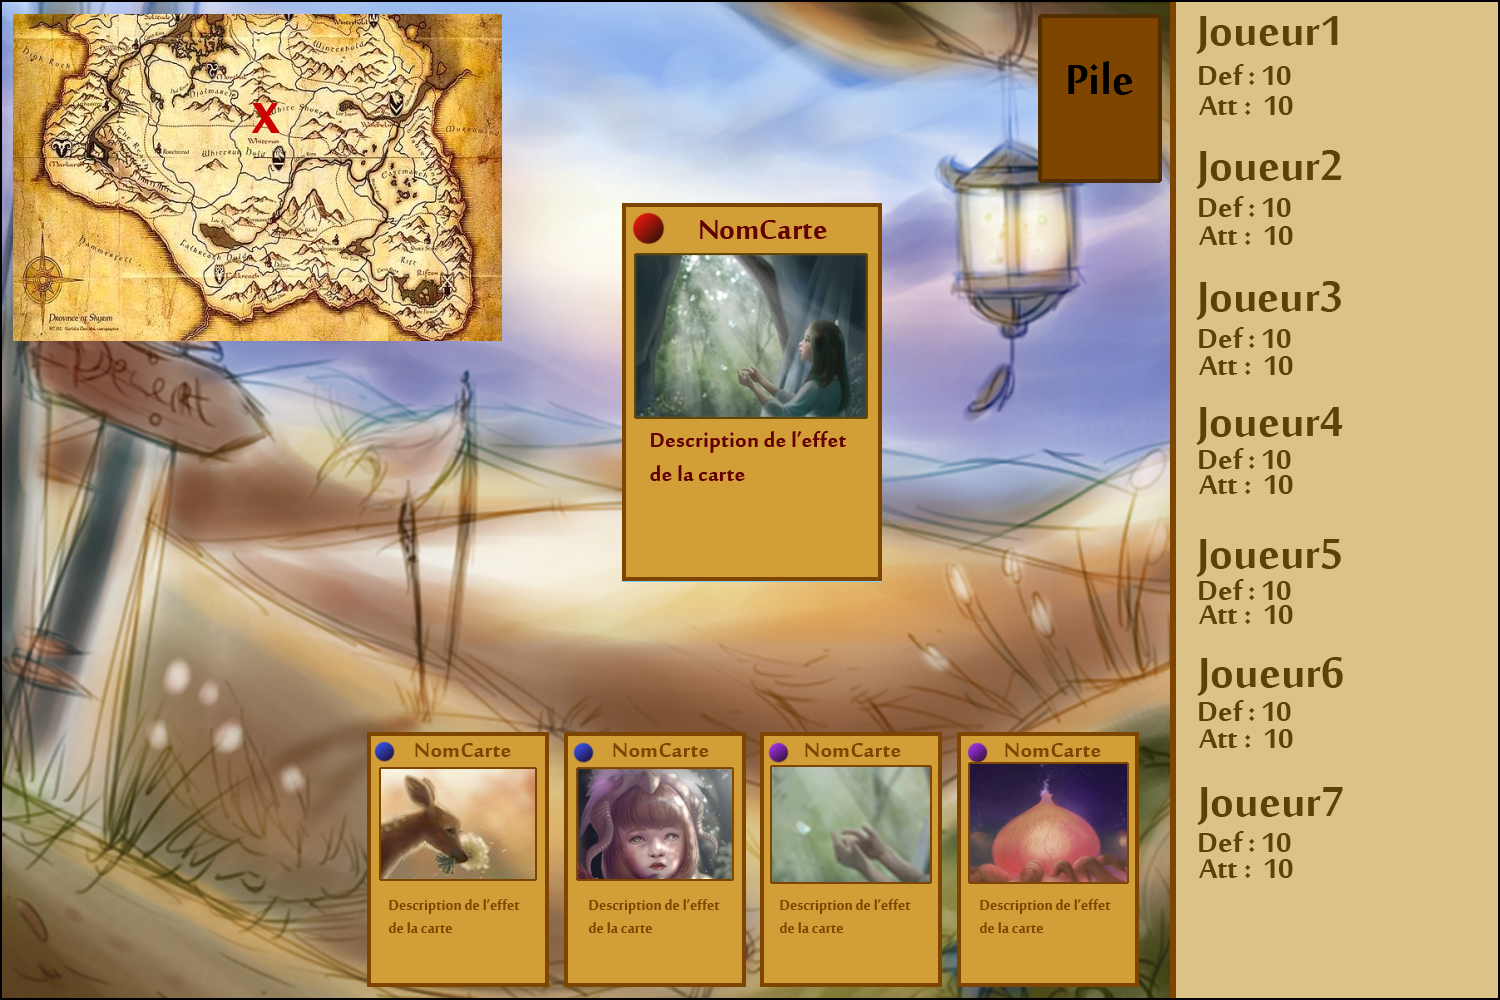
\includegraphics[scale=2.8]{mock-up.png}
	    \caption{Maquette graphique du jeu.}
	    \label{fig:maquette}
    \end{figure}


    \section{Architecture du site}

    \section{Choix des technologies}
    
		Avant de choisir les technologies permettant une implémentation optimale de notre jeu, nous nous sommes penchés tout d'abord sur l'analyse des contraintes de qualité à satisfaire afin d'assurer un déroulement souple de ce dernier. Autrement dit, nous nous sommes aperçus de la nécessité d'établir une communication en temps réel entre les clients utilisant l'application pour assurer un déroulement réaliste et interactif du jeu, aussi bien que du caractère indispensable du paradigme événementiel pour le rendre plus ergonomique et dynamique. De plus, vu qu'il s'agit d'un jeu, en particulier d'un jeu de société, l'intégration des effets graphiques pour l'animer et le rendre le plus élégant possible paraît évident, voire même trivial.

		Ainsi, pour assurer la réalisation de ces contraintes, nous avons choisi JavaScript comme seul langage de programmation pour développer notre jeu ce qui a plus ou moins réduit la durée de notre apprentissage. Effectivement, l'abondance des fonctionnalités fournies par ce langage permet une implémentation JavaScript pure englobant la totalité de l'architecture client-serveur de notre jeu. En réalité, JavaScript a progressé d'un langage web objet/événementiel incontournable conçu pour la dynamisation des pages web du côté client (manipulation du DOM, la bibliothèque jQuery) en un véritable outil omnipotent avec l'arrivée de NodeJS. En réalité, le modèle non-bloquant avec les fonctions de callback caractérisant NodeJS permet une communication extrêmement rapide sur un thread unique entre le serveur et les clients.

		NodeJS intègre aussi la technologie WebSocket dans le module socket.io. Il s'agit d'une API (Application Programming Interface) JavaScript permettant un échange bilatéral synchrone entre les clients et le serveur, contrairement aux serveurs web classiques tels que Apache où la communication se déroule normalement d'une façon asynchrone. Cette caractéristique de WebSocket la rend idéale pour des applications nécessitant une communication en temps réel entre les clients comme la nôtre.

		Outre cela, l'API JavaScript D3 offre une myriade de fonctionnalités permettant la mise en \oe{}uvre d'animations, entre autres, notamment avec des éléments SVG, ce qui la rend parfaite pour assurer le respect de la contrainte de qualité relative à l'aspect esthétique du jeu.

    \section{Base de données}
		Pour stocker les cartes, ainsi que les différentes données cartographiques du jeu, nous nous sommes servis de la notation JSON, un concept fondamental dans le cadre du JavaScript et un moyen très efficace pour la manipulation, le transfert, et le stockage des données.

		Outre l'objet modélisant les cartes du jeu, la notation JSON adoptée pour les hexagones cartographiques est composé de trois chaînes de caractères : un identifiant dénotant les coordonnées de l'hexagone, un environnement indiquant le type du plan dans lequel se déroule le jeu tel qu'une rivière par exemple, et un chemin indiquant l'emplacement de l'image du fond correspondant à l'environnement.

		Pour manipuler, transférer et stocker les données nous avons utilisé le SGBD (Système de Gestion de Bases de Données) offert par MongoDB qui s'avère bien pratique dans le cadre d'une architecture de développement purement basée sur JavaScript telle que la nôtre. En effet, NodeJS offre un module contenant une multitude de fonctionnalités permettant d'interagir aisément avec les bases de données gérées par MongoDB, ce qui facilite énormément la connexion à la base données et la manipulation des données qui y sont stockées.

		MongoDB permet la création de plusieurs bases de données regroupant chacune les données sous forme de \textit{collections} (concept approximatif équivalent à la notion de \textit{tables} dans le cadre d'un modèle de base de données relationnel), contenant chacune des \textit{documents} désignant les objets JSON reflétant nos données.

		MongoDB n'utilise pas le langage de requêtes SQL pour gérer les interactions avec la base de données. Toutefois, le langage de requêtes utilisé reste bien facile à maîtriser et puissant pour couvrir une grande gamme de fonctionnalités nécessaires pour une gestion efficace des données.

		Par conséquent, nous avons créé une base données dans laquelle nous avons stocké nos données en deux collections: une pour stocker les cartes, et l'autre pour stocker les données cartographiques. (Voir figure \ref{fig:schemaBDD})

		\begin{figure}
			\centering
			\begin{tikzpicture}[node distance=6.5cm]
			  \node[entity] (card) {Card};
			  \node[attribute] (id) [above=of card] {\underline{Id}} edge (card);
			  \node[attribute] (type) [above right=of card] {Type} edge (card);
				\node[attribute] (category) [above left=of card] {Category} edge (card);
				\node[attribute] (path) [below right=of card] {Path} edge (card);
				\node[attribute] (action) [below left=of card] {Action} edge (card);

			  \node[entity] (maptiles) [right=of card] {MapTiles};
				\node[attribute] (id) [above=of maptiles] {\underline{Id}} edge (maptiles);
			  \node[attribute] (environment) [below right=of maptiles] {Environment} edge (maptiles);
				\node[attribute] (background) [below left=of maptiles] {Background} edge (maptiles);
			\end{tikzpicture}
			\caption{Modèle EA}
			\label{fig:schemaBDD}
		\end{figure}

\chapter{Développement}

    \section{Gestion de l'événementiel}

    \section{Graphismes}
	    
	    Aidés par les artistes avec lesquels nous avons collaboré, nous avons entièrement réalisé les graphismes de notre jeu, avant d'implémenter l'affichage de ceux-ci. Un travail collaboratif donc, que nous allons détailler dans cette partie. 

        \subsection{Réalisation des images}

        Afin d'obtenir un rendu esthétique pour le jeu, nous avons créé des illustrations avec l'aide des illustrateurs avec lesquels nous avons collaboré. Ceux-ci se sont chargés de faire les fonds pour les environnements plaine et rivière, ainsi que les deux épées présentes sur les cartes du jeu.

        \begin{figure}[h!]
	       	\centering
           	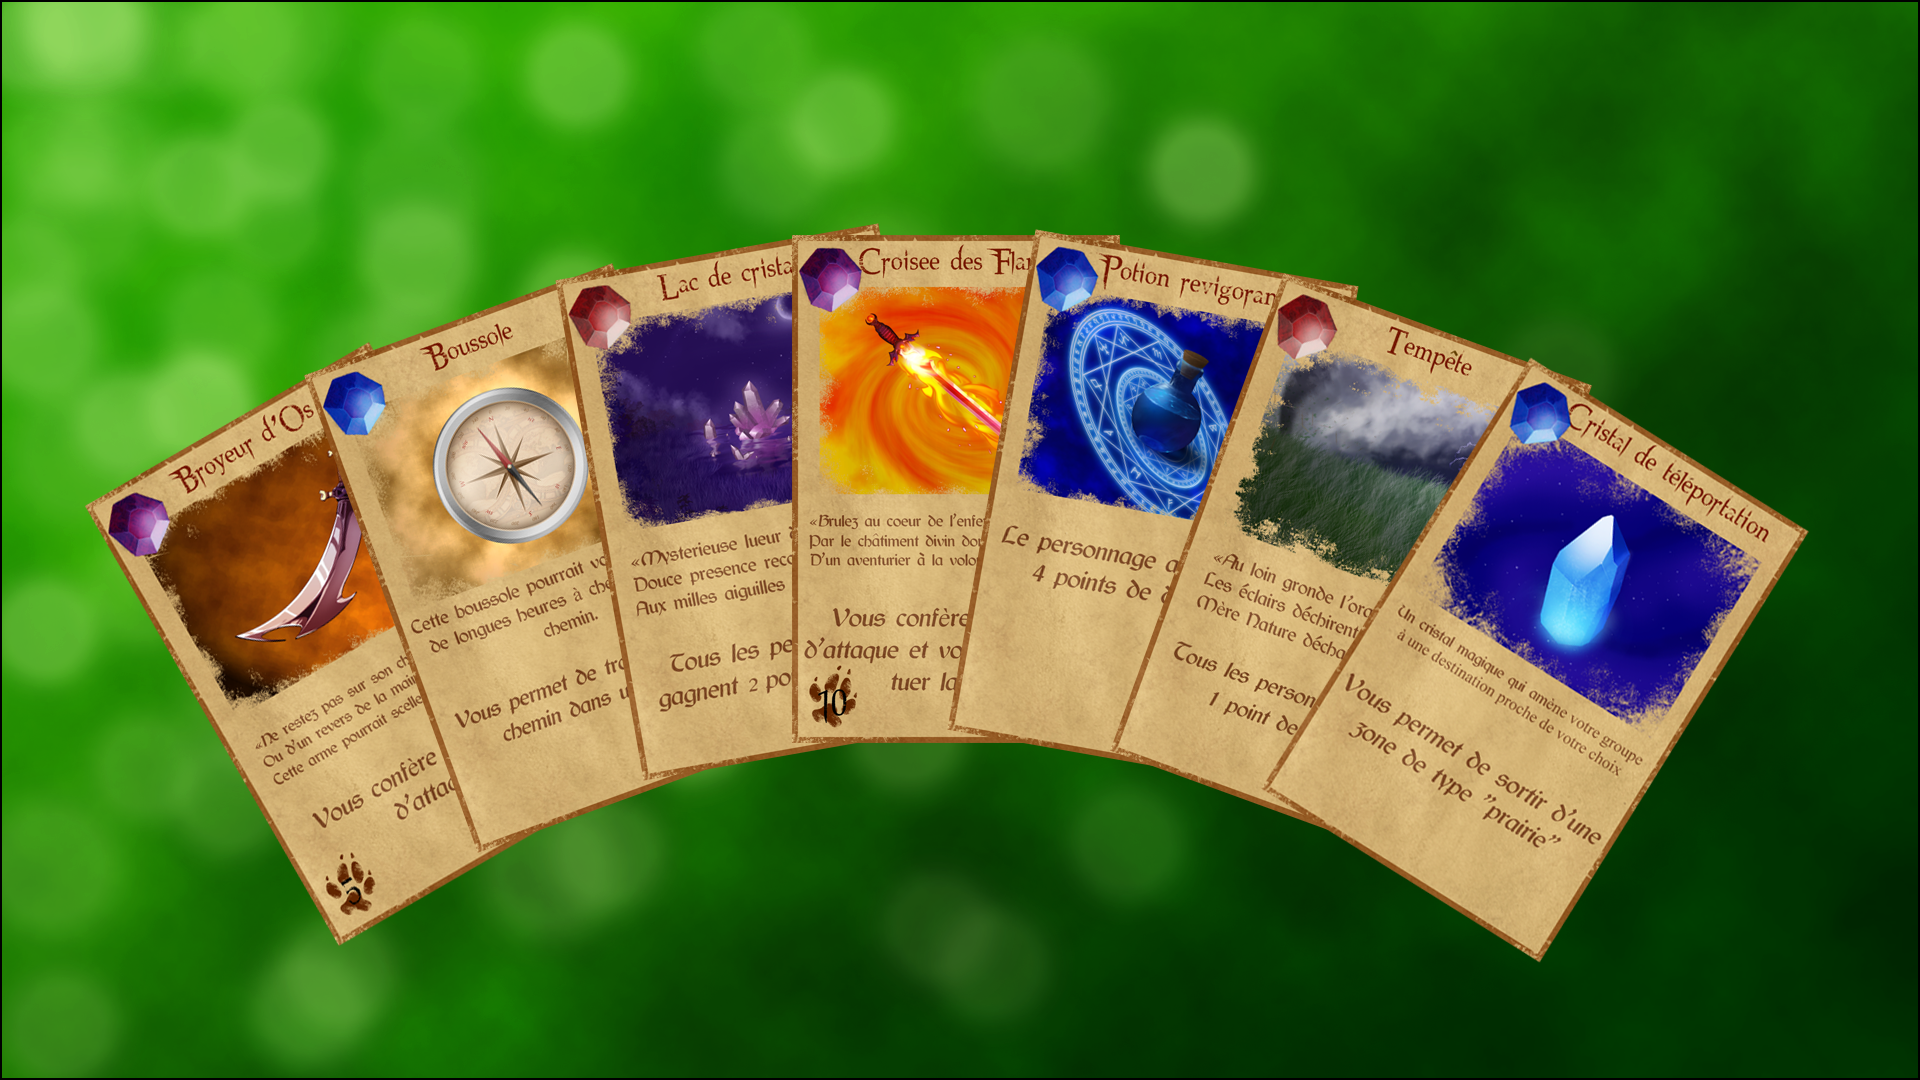
\includegraphics[scale=0.45]{cards.png}
           	\caption{Exemple de cartes crées ainsi que le fond du site.}
           	\label{fig:cartes}
        \end{figure}

        Nous nous sommes chargés de réaliser, à l'aide d'un logiciel de dessin assisté, les autres illustrations pour les cartes, les éléments de décoration des cartes (gemme indiquant le type, symboles d'attaque et de défense, effets visuels. Voir figure \ref{fig:cartes}), le fond pour l'environnement "forêt", le dos de carte pour la pile, ainsi que les autres éléments décoratifs du site (texture de bois, fond).

        Chaque illustration nous a demandé plusieurs heures de travail, et il était prévu que nos collaborateurs réalisent la majeure partie des graphismes. Cependant, par manque de temps de leur part, nous avons dû investir plus de temps que prévu dans cette partie du projet.


        \subsection{Affichage graphique en JavaScript}

        Pour afficher les différents éléments du jeu (cartes de jeu, pile, carte de la zone) nous avons utilisé la bibliothèque D3. Celle-ci permet de manipuler des éléments SVG (Scalable Vector Graphics, format d'images vectorielles).

        Nous avons créé une zone SVG recouvrant toute la partie du site dédiée au jeu, de la manière suivante :

        \begin{verbatim}
        var svg = d3.select('#svgWin')
                    .append('svg')
                    .attr('width', 900)
                    .attr('height', 650);
        \end{verbatim}

        Ici, 'svgWin' désigne la balise html <div> ayant pour attribut "id = 'svgWin' ". La fonction append('svg') permet de créer un élément SVG fils de "svgWin". Nous lui attribuons ensuite une largeur et une hauteur correspondant à la taille de la zone dédiée au jeu. Nous avons procédé de la même manière pour les images, avec des objets de type "svg:image", en y ajoutant les attributs "x" et "y" pour la position dans la zone SVG.

        Outre l'affichage d'image, nous avons également affiché la carte des zones du jeu à l'aide de D3 (voir figure \ref{fig:map}). Pour cela, nous avons créé des hexagones que nous avons rempli de couleurs correspondant à l'environnement de la zone représentée par chaque hexagone. Le dessin des hexagones est réalisé à l'aide de "path", qui permet de dessiner les contours d'une forme (rectangle, cercle, simple ligne...). La position sur la carte, qui se déplace lorsque les joueurs changent de lieu, est marquée par un cercle. 
        
		\begin{figure}[h!]
			\centering
			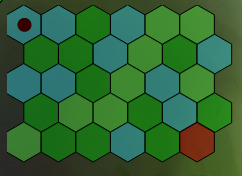
\includegraphics[scale=0.95]{map}
			\label{fig:map}
			\caption{La carte des zones du jeu implémentée en JavaScript (D3)}
		\end{figure}

        Nous avons également utilisé D3 pour effectuer un zoom sur les cartes en main lors du passage de la souris sur celles-ci (voir figure \ref{fig:zoom})afin que les joueurs puissent lire les effets de leurs cartes plus facilement.
        
		\begin{figure}[h!]
			\centering
			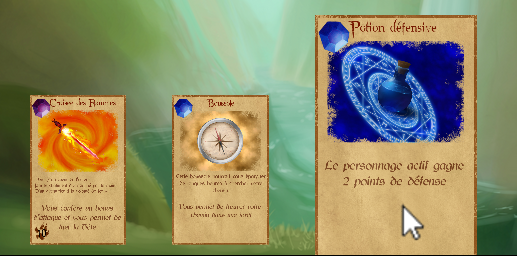
\includegraphics[scale=0.6]{zoom}
			\label{fig:zoom}
			\caption{Le zoom effectué lorsque la souris est passée sur une carte de la main}
		\end{figure}


\chapter{Manuel d'utilisation}

    \section{Navigation sur le site}

    Le site comporte 3 différentes pages, accessibles depuis la barre de menu en haut (voir 1 figure \ref{fig:menu}). La page principale est celle concernant uniquement le jeu, avec en haut à gauche le champ de texte pour entrer un pseudo et se connecter, ainsi que le bouton permettant de quitter la partie (voir 2 figure \ref{fig:manual})). Au centre de la page se trouve la fenêtre de jeu.

    Il est possible de consulter les règles du jeu en cliquant sur le lien "Règles" dans le menu. On y trouve toutes les informations nécessaires pour une partie.

    Enfin, tous les contributeurs du projet (les artistes ayant collaboré avec nous ainsi que nous-mêmes) sont listés sur la page "crédits", également accessible à l'aide du lien du même nom dans le menu.

    \section{Fonctionnement du jeu}

    Une fois la partie commencée, chaque joueur joue tour à tour. Un tour consiste à tirer une carte de la pile, en cliquant sur l'image du dos de carte sur la gauche de la fenêtre de jeu (voir 3 figure \ref{fig:manual}). Le joueur peut alors décider de prendre la carte ou la jeter, en cliquant sur le bouton correspondant qui s'affichera en même temps que la carte tirée, qui sera affichée au centre de l'écran (voir 4 figure \ref{fig:manual}).

    Les cartes que le joueur décide de prendre s'affichent en bas de la fenêtre de jeu (voir 5 figure \ref{fig:manual}). La main du joueur est limitée à cinq cartes, par conséquent, si l'on a déjà une main pleine on ne peut pas prendre de nouvelle carte sans se débarrasser d'une autre. Différentes interactions sont possibles avec les cartes que l'on a en main : en cliquant sur une carte, des choix s'offrent à nous, modélisés par des boutons. S'il s'agit d'une carte équipable, on peut l'équiper. S'il s'agit d'une carte utilisable (potion ou objet permettant de changer de lieu), on peut l'utiliser. Dans tous les cas, il est possible de jeter la carte si on décide qu'elle ne nous est plus d'aucune utilité ou que l'on souhaite faire de la place dans notre main.
    
	\begin{figure}[h!]
		\centering
		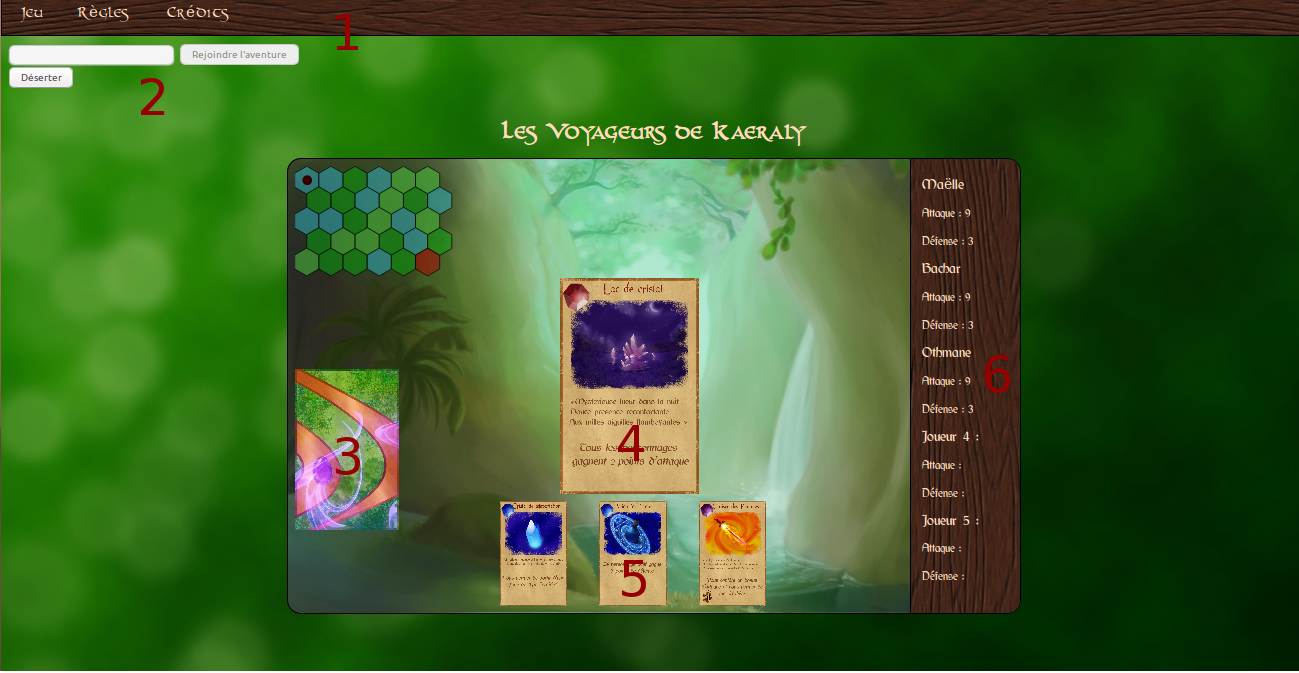
\includegraphics[scale=0.35]{manual}
		\label{fig:manual}
		\caption{Aperçu de la page du jeu et ses différents éléments.}
	\end{figure}

    Dans le cas de l'utilisation d'un objet permettant de changer de zone, il faut choisir la zone suivante dans laquelle les joueurs veulent se placer. Il est impossible de reculer, seules trois directions sont possibles : haut, droite, bas.

    Un joueur dispose d'un temps imparti pour terminer son tour. Il est possible de passer son tour après avoir réalisé toutes les actions que l'on souhaitait faire en cliquant sur le bouton "Terminer le tour". Si le joueur ne clique pas sur ce bouton dans les temps, le tour passe automatiquement au joueur suivant afin d'éviter que la partie ne soit bloquée par un joueur inactif.
    
    Les cartes équipables ainsi que les potions permettent de modifier les statistiques de défense et/ou d'attaque d'un joueur. Celles-ci sont visibles sur le côté droit de la fenêtre de jeu (voir 6 figure \ref{fig:manual}).

\chapter*{Conclusion}
\addcontentsline{toc}{chapter}{Conclusion}

    \section*{Bilan}
    \addcontentsline{toc}{section}{Bilan}

    \section*{Perspectives}
    \addcontentsline{toc}{section}{Perspectives}

    \section*{Apports personnels du projet}
    \addcontentsline{toc}{section}{Apports personnels du projet}

\end{document}
